\documentclass{beamer}

%%%%%%%%%%%%%%%%%%%%%%%%%%%%%%%%%%%%%%%%%%%%%%%%%%%%%%%%%%%%%%%%%%%%%%%%%%%%%%%%
% Packages
%%%%%%%%%%%%%%%%%%%%%%%%%%%%%%%%%%%%%%%%%%%%%%%%%%%%%%%%%%%%%%%%%%%%%%%%%%%%%%%%

% Warn about commands, classes and packages that are outdated and superseded.
% Orthodox checks for pitfalls that are not technically incorrect.
%\usepackage[l2tabu,orthodox,abort]{nag}
\usepackage[l2tabu,orthodox]{nag}

% For font and input encoding.
\usepackage[utf8]{inputenc}
%\usepackage[T1]{fontenc}

% Pretty much all of the ams maths packages.
\usepackage{amsmath,amsthm,amssymb,amsfonts}

% Allows inclusion of graphics easily and "configurably".
\usepackage{graphicx}

% Typesets URLs sensibly --- with a TrueType font, hyperlinked in PDFs, and not
% breaking across lines.
\usepackage{url}

% Count the number of used registers (counter, dimen, skip, muskip, box, token,
% input, output, math families, languages, insertions). Also time the amount of
% time required for LaTeX compilation.
\usepackage[timer,left]{regstats}

% The listings package is a source code printer for LaTeX. You can typeset stand
% alone files as well as listings with an environment similar to verbatim as
% well as you can print code snippets using a command similar to \verb.
\usepackage{listings}

% This package implements high-level interface commands for class file writers
% which allows the separation of formatting commands (typically instances of
% so-called `templates') and their arguments from the signature of
% document-level commands.
\usepackage{xparse}

% This package allows verbatim text to be typeset in bold.
\usepackage{alltt}
\renewcommand{\ttdefault}{txtt}

% This style option improves the interface for defining floating objects such
% as figures and tables in LaTeX. It adds the notion of a `float style' that
% governs appearance of floats. New kinds of floats may be defined using a
% \newfloat command analogous to \newtheorem. This style option also
% incorporates the functionality of David Carlisle's style option here, giving
% floating environments a [H] option which means `PUT IT HERE' (as opposed to
% the standard [h] option which means `You may put it here if you like').
\usepackage{float}

% This is the style file for the gnuplot PGF/TikZ terminal. It is associated
% with the 'gnuplot.lua' script.
\usepackage{gnuplot-lua-tikz}

% The caption package provides many ways to customise the captions in floating
% environments such figure and table.
\usepackage{caption}

% This package supports typesetting of sub-captions (by using the the
% sub-caption feature of the caption package).
\usepackage{subcaption}

% This package reimplements the LATEX verbatim and verbatim* environments. In
% addition it provides a comment environment that skips any commands or text
% between \begin{comment} and the next \end{comment}. It also defines the
% command verbatim to input a whole file verbatim.
\usepackage{verbatim}

% TODO
\usepackage[noline,ruled]{algorithm2e}

% TODO
\usepackage{pgfplots}
\usepackage{tikz}\usetikzlibrary{positioning,shapes,shadows,arrows}

% For \ifthenelse command
\usepackage{ifthen}

% For \maxsizebox command
\usepackage{adjustbox}

% My custom packages
\usepackage{escape,persons,pgf-pie}

%%%%%%%%%%%%%%%%%%%%%%%%%%%%%%%%%%%%%%%%%%%%%%%%%%%%%%%%%%%%%%%%%%%%%%%%%%%%%%%%
% Beamer configuration.
%%%%%%%%%%%%%%%%%%%%%%%%%%%%%%%%%%%%%%%%%%%%%%%%%%%%%%%%%%%%%%%%%%%%%%%%%%%%%%%%
% Presentation mode
\mode<presentation>

% Load a theme
\usetheme{Warsaw}
%\useoutertheme[footline=authortitle]{miniframes}
\useoutertheme{smoothbars}

% For animations in beamer
\usepackage{multimedia}

% Reduce the font size of captions
\setbeamerfont{caption}{size=\scriptsize}

% Show notes
\setbeameroption{show notes}
%\setbeameroption{show only notes}
%\setbeameroption{hide notes}
%\usepackage{pgfpages}\setbeameroption{show notes on second screen}

% Hide navigation symbols
%\setbeamertemplate{navigation symbols}{}

%%%%%%%%%%%%%%%%%%%%%%%%%%%%%%%%%%%%%%%%%%%%%%%%%%%%%%%%%%%%%%%%%%%%%%%%%%%%%%%%
% Custom colours
%%%%%%%%%%%%%%%%%%%%%%%%%%%%%%%%%%%%%%%%%%%%%%%%%%%%%%%%%%%%%%%%%%%%%%%%%%%%%%%%
\definecolor{darkGreen}{rgb}{0,0.6,0}
\definecolor{gray}{rgb}{0.5,0.5,0.5}
\definecolor{mauve}{rgb}{0.58,0,0.82}
\definecolor{brightGreen}{rgb}{0,1,0}

%%%%%%%%%%%%%%%%%%%%%%%%%%%%%%%%%%%%%%%%%%%%%%%%%%%%%%%%%%%%%%%%%%%%%%%%%%%%%%%%
% Source code formatting
%%%%%%%%%%%%%%%%%%%%%%%%%%%%%%%%%%%%%%%%%%%%%%%%%%%%%%%%%%%%%%%%%%%%%%%%%%%%%%%%
% Default settings
\lstset{
    basicstyle=\ttfamily,           % font
                                    %
    title=\lstname,                 % show the filename of files included with \lstinputlisting
    captionpos=b,                   % sets the caption-position to bottom
    backgroundcolor=\color{white},  % choose the background color
                                    %
    numbers=left,                   % where to put the line-numbers
    numberstyle=\tiny\color{gray},  % the style that is used for the line-numbers
    stepnumber=1,                   % the step between two line-numbers
    numbersep=5pt,                  % how far the line-numbers are from the code
                                    %
    showspaces=false,               % show spaces adding particular underscores
    showstringspaces=false,         % underline spaces within strings
    showtabs=false,                 % show tabs within strings adding particular underscores
    tabsize=4,                      % sets default tabsize
    breaklines=true,                % sets automatic line breaking
    breakatwhitespace=false,        % sets if automatic breaks should only happen at whitespace
                                    %
    keywordstyle=\color{blue},      % keyword style
    commentstyle=\color{darkGreen}, % comment style
    stringstyle=\color{mauve},      % string literal style
    escapeinside={\%*}{*)},         % if you want to add a comment within your code
    morekeywords={*,...}            % if you want to add more keywords to the set
}
\lstloadlanguages{C,Matlab}

%%%%%%%%%%%%%%%%%%%%%%%%%%%%%%%%%%%%%%%%%%%%%%%%%%%%%%%%%%%%%%%%%%%%%%%%%%%%%%%%
% Variables (to save retyping and reformatting these throughout the document).
%%%%%%%%%%%%%%%%%%%%%%%%%%%%%%%%%%%%%%%%%%%%%%%%%%%%%%%%%%%%%%%%%%%%%%%%%%%%%%%%
%%%%%%%%%%%%%%%%%%%%%%%%%%%%%%%%%%%%%%%%%%%%%%%%%%%%%%%%%%%%%%%%%%%%%%%%%%%%%%%%
% Variables (to save retyping and reformatting these throughout the document).
%%%%%%%%%%%%%%%%%%%%%%%%%%%%%%%%%%%%%%%%%%%%%%%%%%%%%%%%%%%%%%%%%%%%%%%%%%%%%%%%
\usepackage{definevariable} % for \defineVariable
\usepackage{persons} % for \definePerson, \getPerson, \formatPerson

\defineVariable\thesis{}{Thesis}
\defineVariable\thesisTitle{\textsc}{Implementation of Random Projection Algorithms Using an FPGA}
\defineVariable\thesisDate{}{2012}
\defineVariable\studentName{\formatPerson}{\getPerson*{Spence}}
\defineVariable\supervisorName{\formatPerson}{\getPerson*{Leong}}

\defineVariable\degreeName{}{Bachelor of Engineering (Computer)}
\defineVariable\schoolName{}{School of Electrical Engineering}
\defineVariable\studentID{}{308216350}
\defineVariable\universityName{}{The University of Sydney}
\defineVariable\uosAssessment{}{\thesis}
\defineVariable\uosCode{}{ELEC4712/ELEC4713}

\urldef{\gitRepoHTTP}\url{https://github.com/joshuaspence/ThesisCode.git}
\urldef{\gitRepoSSH}\url{git@github.com:joshuaspence/ThesisCode.git}

% People
\definePerson{Chawla}{Sanjay Chawla}
\definePerson{Frechtling}{Michael Frechtling}
\definePerson{Heinrichs}{Amelia Heinrichs}
\definePerson{Khoa}{Nguyen Lu Dang Khoa}
\definePerson{Leong}{Philip Leong}
\definePerson{Spence}{Joshua Spence}

% PDF metadata
\newcommand*\pdfmetadata{%
    pdfauthor={Joshua Spence},
    pdftitle={Implementation of Random Projection Algorithms Using an FPGA},
    pdfsubject={},
    pdfkeywords={commute time,anomaly detection,FPGA},
    pdfdisplaydoctitle={true}
}

% Copyrights and trademarks
\newcommand\ARM{ARM\textsuperscript{\textregistered}}
\newcommand\Cortex{Cortex\textsuperscript{\texttrademark}}
\newcommand\IntelXeon{Intel\textsuperscript{\textregistered} Xeon\textsuperscript{\textregistered}}
\newcommand\IntelCoreiSeven{Intel\textsuperscript{\textregistered} Core\textsuperscript{\texttrademark} i7}
\newcommand\AutoESL{\software{Xilinx\textsuperscript{\textregistered} AutoESL}}
\newcommand\ModelSim{\software{Altera\textsuperscript{\textregistered} ModelSim}}
\newcommand\Xilinx{Xilinx\textsuperscript{\textregistered}}

%%%%%%%%%%%%%%%%%%%%%%%%%%%%%%%%%%%%%%%%%%%%%%%%%%%%%%%%%%%%%%%%%%%%%%%%%%%%%%%%
% Custom commands
%%%%%%%%%%%%%%%%%%%%%%%%%%%%%%%%%%%%%%%%%%%%%%%%%%%%%%%%%%%%%%%%%%%%%%%%%%%%%%%%

%===============================================================================
% Format a block size profiling plot.
%-------------------------------------------------------------------------------
% \blockSizeProfilingPlot{DATASET}
%===============================================================================
\makeatletter
\newcommand\blockSizeProfilingPlot[1]{%
    \def\profilingPlots@width{0.9\textwidth}%
    \def\profilingPlots@height{0.9\textheight}%
    %
    \makebox[\textwidth][c]{%
        \maxsizebox{\profilingPlots@width}{\profilingPlots@height}{%
            \input{plots/block_size/#1}%
        }%
    }%
}
\makeatother

%===============================================================================
% Format a profiling plot.
%-------------------------------------------------------------------------------
% \profilingPlots{DATASET1}{DATASET2}{DATASET3}
%===============================================================================
\makeatletter
\newcommand\profilingPlots[3]{%
    \def\profilingPlots@verticalOffset{\vskip-1.5em}%
    \def\profilingPlots@columnWidth{0.33\textwidth}%
    \def\profilingPlots@pcaWidth{0.9\textwidth}%
    \def\profilingPlots@plotWidth{0.7\textwidth}%
    \def\profilingPlots@legendHeight{0.15\textheight}%
    %
    \profilingPlots@verticalOffset
    \begin{columns}[c]%
        \column{\profilingPlots@columnWidth}%
        \ifthenelse{\equal{#1}{}}{}{
            \begin{figure}%
                \includegraphics[width=\profilingPlots@pcaWidth]{pca/#1}\\%
                \resizebox{\profilingPlots@plotWidth}{!}{\input{plots/c/#1}}%
                \caption{\escape{#1}}%
            \end{figure}%
        }%
        %
        \column{\profilingPlots@columnWidth}%
        \ifthenelse{\equal{#2}{}}{}{
            \begin{figure}%
                \includegraphics[width=\profilingPlots@pcaWidth]{pca/#2}\\%
                \resizebox{\profilingPlots@plotWidth}{!}{\input{plots/c/#2}}%
                \caption{\escape{#2}}%
            \end{figure}%
        }%
        %
        \column{\profilingPlots@columnWidth}%
        \ifthenelse{\equal{#3}{}}{}{
            \begin{figure}%
                \includegraphics[width=\profilingPlots@pcaWidth]{pca/#3}\\%
                \resizebox{\profilingPlots@plotWidth}{!}{\input{plots/c/#3}}%
                \caption{\escape{#3}}%
            \end{figure}%
        }%
    \end{columns}%
    \vfill
    \makebox[\textwidth][c]{%
        \resizebox{!}{\profilingPlots@legendHeight}{%
            \pielegend[bound,color={yellow!60,blue!60,white!60,orange!60}]{
1/\escape{top_n_outlier_pruning_block},
1/\escape{distance_squared},
1/\escape{Other},
1/\escape{add_neighbour}
}
%
        }%
    }%
}
\makeatother

%%%%%%%%%%%%%%%%%%%%%%%%%%%%%%%%%%%%%%%%%%%%%%%%%%%%%%%%%%%%%%%%%%%%%%%%%%%%%%%%
% Custom formatting commands
%%%%%%%%%%%%%%%%%%%%%%%%%%%%%%%%%%%%%%%%%%%%%%%%%%%%%%%%%%%%%%%%%%%%%%%%%%%%%%%%

%===============================================================================
% Format the name of an algorithm.
%-------------------------------------------------------------------------------
% \algm{}
%===============================================================================
\newcommand\algm[1]{\emph{#1}}

%===============================================================================
% Format the name of a command line command. Also allows words to be broken over
% multiple lines
%
% See: http://jevopi.blogspot.com.au/2010/04/latex-lstinline-and-hyphenations.html
%-------------------------------------------------------------------------------
% \command{CMD}
%===============================================================================
\newcommand\command[1]{\lstinline[breaklines,literate={\_}{}{0\discretionary{\_}{}{\_}}]`#1`}

%===============================================================================
% Format the name of a data set.
%-------------------------------------------------------------------------------
% \dataset{DATASET}
%===============================================================================
\newcommand\dataset[1]{`\escape{#1}'}

%===============================================================================
% Format a computer host name.
%-------------------------------------------------------------------------------
% \hostname{HOSTNAME}
%===============================================================================
\newcommand\hostname[1]{\emph{#1}}

%===============================================================================
% Format the name of a programming language.
%-------------------------------------------------------------------------------
% \progLang{LANG}
%===============================================================================
\newcommand\progLang[1]{\lstinline`#1`}

%===============================================================================
% Format the name of a software package.
%-------------------------------------------------------------------------------
% \software{NAME}[CMD]
%===============================================================================
\NewDocumentCommand\software{om}{``#2''\IfNoValueTF{#1}{}{\space(\command{#1})}}

%%%%%%%%%%%%%%%%%%%%%%%%%%%%%%%%%%%%%%%%%%%%%%%%%%%%%%%%%%%%%%%%%%%%%%%%%%%%%%%%
% Graphics directory
%%%%%%%%%%%%%%%%%%%%%%%%%%%%%%%%%%%%%%%%%%%%%%%%%%%%%%%%%%%%%%%%%%%%%%%%%%%%%%%%
\graphicspath{{../img/}}

%%%%%%%%%%%%%%%%%%%%%%%%%%%%%%%%%%%%%%%%%%%%%%%%%%%%%%%%%%%%%%%%%%%%%%%%%%%%%%%%
% Glossary
%%%%%%%%%%%%%%%%%%%%%%%%%%%%%%%%%%%%%%%%%%%%%%%%%%%%%%%%%%%%%%%%%%%%%%%%%%%%%%%%
\usepackage[toc,xindy]{glossaries} % note that hyperref must be loaded first
\makeglossaries
\loadglsentries{acronym}

%%%%%%%%%%%%%%%%%%%%%%%%%%%%%%%%%%%%%%%%%%%%%%%%%%%%%%%%%%%%%%%%%%%%%%%%%%%%%%%%
% Bibliography
%%%%%%%%%%%%%%%%%%%%%%%%%%%%%%%%%%%%%%%%%%%%%%%%%%%%%%%%%%%%%%%%%%%%%%%%%%%%%%%%
\usepackage[backend=bibtex,language=australian]{biblatex} % use biblatex instead of bibtex
\bibliography{thesis}

%%%%%%%%%%%%%%%%%%%%%%%%%%%%%%%%%%%%%%%%%%%%%%%%%%%%%%%%%%%%%%%%%%%%%%%%%%%%%%%%
%                               END OF PREAMBLE                                %
%%%%%%%%%%%%%%%%%%%%%%%%%%%%%%%%%%%%%%%%%%%%%%%%%%%%%%%%%%%%%%%%%%%%%%%%%%%%%%%%
\begin{document}

%%%%%%%%%%%%%%%%%%%%%%%%%%%%%%%%%%%%%%%%%%%%%%%%%%%%%%%%%%%%%%%%%%%%%%%%%%%%%%%%
% Title Page
%%%%%%%%%%%%%%%%%%%%%%%%%%%%%%%%%%%%%%%%%%%%%%%%%%%%%%%%%%%%%%%%%%%%%%%%%%%%%%%%
\pdfbookmark[0]{Title}{titlepage}
\frame[label=titlepage,shrink]{\titlepage}

%%%%%%%%%%%%%%%%%%%%%%%%%%%%%%%%%%%%%%%%%%%%%%%%%%%%%%%%%%%%%%%%%%%%%%%%%%%%%%%%
% Introduction
%%%%%%%%%%%%%%%%%%%%%%%%%%%%%%%%%%%%%%%%%%%%%%%%%%%%%%%%%%%%%%%%%%%%%%%%%%%%%%%%
\section{Introduction}
%%%%%%%%%%%%%%%%%%%%%%%%%%%%%%%%%%%%%%%%%%%%%%%%%%%%%%%%%%%%%%%%%%%%%%%%%%%%%%%%
% Overview
%%%%%%%%%%%%%%%%%%%%%%%%%%%%%%%%%%%%%%%%%%%%%%%%%%%%%%%%%%%%%%%%%%%%%%%%%%%%%%%%
% Briefly tell the audience what you are going to cover.
\subsection{Overview}
\begin{frame}[label=overview]{Overview}
    \begin{itemize}
        \item Anomaly detection algorithm using commute time and Eigenspace
            approximation.
        \item Software-hardware coprocessing.
        \item Hardware implementation.
        \item A bullet on FPGAs.
        \item Reconfigurable computing is the application of FPGAs to computing problems.
    \end{itemize}
\end{frame}

%%%%%%%%%%%%%%%%%%%%%%%%%%%%%%%%%%%%%%%%%%%%%%%%%%%%%%%%%%%%%%%%%%%%%%%%%%%%%%%%
% Motivation
%%%%%%%%%%%%%%%%%%%%%%%%%%%%%%%%%%%%%%%%%%%%%%%%%%%%%%%%%%%%%%%%%%%%%%%%%%%%%%%%
% Briefly tell the audience why you are doing your research. Sell your audience
% on why your topic is important and of interest to them.
\subsection{Motivation}
\begin{frame}[label=motivation]{Motivation}
    \begin{itemize}
        \item The amount of data being collected and stored is continually
            increasing.
        \item Anomaly detection is an important technique which can be applied
            to a wide range of applications.
    \end{itemize}
\end{frame}

\begin{frame}[label=applications]{Applications}
    \begin{itemize}
        \item Stock market analysis
        \item Network intrusion detection
        \item Image comparison
        \item Fraud detection
        \item Data cleaning
        \item Detecting employers with poor injury histories
    \end{itemize}
\end{frame}

%%%%%%%%%%%%%%%%%%%%%%%%%%%%%%%%%%%%%%%%%%%%%%%%%%%%%%%%%%%%%%%%%%%%%%%%%%%%%%%%
% Aims
%%%%%%%%%%%%%%%%%%%%%%%%%%%%%%%%%%%%%%%%%%%%%%%%%%%%%%%%%%%%%%%%%%%%%%%%%%%%%%%%
% This section should be short and memorable.
\subsection{Aims}
\begin{frame}[label=aims]{Aims}
    The aim of this \thesis{} is to \emph{investigate the performance benefits}
    that can be obtained by \emph{applying reconfigurable computing design
    principles} to an \emph{anomaly detection algorithm} using commute time and
    Eigenspace sampling.
\end{frame}

%%%%%%%%%%%%%%%%%%%%%%%%%%%%%%%%%%%%%%%%%%%%%%%%%%%%%%%%%%%%%%%%%%%%%%%%%%%%%%%%
% Contributions
%%%%%%%%%%%%%%%%%%%%%%%%%%%%%%%%%%%%%%%%%%%%%%%%%%%%%%%%%%%%%%%%%%%%%%%%%%%%%%%%
% What I contributed towards this research area.
\subsection{Contributions}
\begin{frame}[label=contributions]{Contributions}
    \begin{enumerate}
        \item Quantitative analysis and benchmarking of the properties of the
            chosen anomaly detection algorithm.
        \begin{itemize}
            \item Justify why we worked on that.
        \end{itemize}
        \item An architecture for accelerating a wide class of algorithms.
        \begin{itemize}
            \item Other examples of where this design could be applied.
        \end{itemize}
        \item Implementation
    \end{enumerate}
\end{frame}

%%%%%%%%%%%%%%%%%%%%%%%%%%%%%%%%%%%%%%%%%%%%%%%%%%%%%%%%%%%%%%%%%%%%%%%%%%%%%%%%
% The Algorithm
%%%%%%%%%%%%%%%%%%%%%%%%%%%%%%%%%%%%%%%%%%%%%%%%%%%%%%%%%%%%%%%%%%%%%%%%%%%%%%%%
\section{The Algorithm}
%%%%%%%%%%%%%%%%%%%%%%%%%%%%%%%%%%%%%%%%%%%%%%%%%%%%%%%%%%%%%%%%%%%%%%%%%%%%%%%%
% The Algorithm
%%%%%%%%%%%%%%%%%%%%%%%%%%%%%%%%%%%%%%%%%%%%%%%%%%%%%%%%%%%%%%%%%%%%%%%%%%%%%%%%
\subsection{The Algorithm}
\begin{frame}{The Algorithm}{Anomaly Detection Using Commute Time}\relax
    {\tiny
        \begin{algorithm}[H]
            % TODO
\LinesNumbered

\SetKwInput{InputK}{k}
\SetKwInput{InputN}{N}
\SetKwInput{InputD}{Data}
\SetKwInOut{OutputO}{outliers}

\InputK{the number of nearest neighbors}
\InputN{the number of outliers to return}
\InputD{a set of examples in random order}
\OutputO{a set of outliers}

\SetKwData{varB}{b}
\SetKwData{Block}{block}
\SetKwData{Cutoff}{cutoff}
\SetKwData{varD}{d}
\SetKwData{Data}{Data}
\SetKwData{varK}{k}
\SetKwData{varN}{N}
\SetKwData{Neighbours}{neighbours}
\SetKwData{varO}{o}
\SetKwData{Outliers}{outliers}
\SetKwData{Score}{score}

\SetKwFunction{Closest}{closest}
\SetKwFunction{Distance}{distance}
\SetKwFunction{GetNextBlock}{getNextBlock}
\SetKwFunction{MaxDist}{maxDist}
\SetKwFunction{Min}{min}
\SetKwFunction{Top}{top}

\Begin{
    $\Cutoff \longleftarrow 0$\tcp*[l]{set the cutoff for pruning to $0$}
    $\Outliers \longleftarrow \emptyset$\tcp*[l]{initialize to the empty set}
    \BlankLine
    \While(\tcp*[h]{load a block of examples from \varD}){$\Block \longleftarrow \GetNextBlock{\Data}$}{
        $\Neighbours(\varB) \longleftarrow \emptyset, \quad \forall \, \varB \in \Block$\;
        \BlankLine
        \ForEach{$\varD \in \Data$}{
            \ForEach{$\varB \in \Block \: : \: \varB \neq \varD$}{
                \If{$|\Neighbours(\varB)| < \varK \: \lor \: \Distance{\varB, \varD} < \MaxDist{\varB, \Neighbours(\varB)}$}{
                    $\Neighbours(\varB) \longleftarrow \Closest{\varB, \Neighbours(\varB)} \cup \varD, \varK)$\;
                    \If{$\Score(\Neighbours(\varB), \varB) < \Cutoff$}{
                        $\Block \longleftarrow \Block \setminus \varB$\;
                    }
                }
            }
        }
        \BlankLine
        $\Outliers \longleftarrow $\Top{$\Block \cup \Outliers$, $\varN$}\tcp*[l]{keep only the top n outliers}
        $\Cutoff \longleftarrow \Min_{\varO \in \Outliers}(\Score(\varO))$\tcp*[l]{the cutoff is the score of the weakest outlier}
    }
    \KwRet{\Outliers}\;
}

        \end{algorithm}
    }
\end{frame}

\begin{frame}[shrink]{The Algorithm}{Outlier Pruning}\relax
    {\tiny
        \begin{algorithm}[H]
            \LinesNumbered

\SetKwInput{InputK}{k}\InputK{the number of nearest neighbours to consider}
\SetKwInput{InputN}{N}\InputN{the number of outliers to return}
\SetKwInput{InputData}{data}\InputData{a set of examples in random order}
\SetKwInOut{Output}{outliers}\Output{a set of outliers}
\SetKwInOut{OutputScores}{outlier\_scores}\OutputScores{}

\SetKwData{BlockIterator}{b}
\SetKwData{Block}{block}
\SetKwData{Cutoff}{cutoff}
\SetKwData{DataIterator}{d}
\SetKwData{Data}{data}
\SetKwData{NumK}{k}
\SetKwData{NumN}{N}
\SetKwData{Neighbours}{neighbours}
\SetKwData{OutlierIterator}{o}
\SetKwData{Outliers}{outliers}
\SetKwData{Score}{score}

\SetKwFunction{Closest}{closest}
\SetKwFunction{Distance}{distance}
\SetKwFunction{LoadBlock}{load\_next\_block}
\SetKwFunction{MaxDist}{max\_dist}
\SetKwFunction{Min}{min}
\SetKwFunction{Top}{top}

\Begin{
    \Cutoff $\leftarrow$ 0\tcp*[l]{set the cutoff for pruning to $0$}
    \Outliers $\leftarrow\emptyset$\tcp*[l]{initialize to the empty set}
    \BlankLine
    \While(\tcp*[h]{load a block of examples from \Data}){\Block $\leftarrow$ \LoadBlock{\Data}}{
        \ForEach{\BlockIterator $\in$ \Block}{
            $\Neighbours[\BlockIterator]\leftarrow\emptyset$\;
        }
        \BlankLine
        \ForEach{\DataIterator $\in$ \Data}{
            \ForEach{\BlockIterator $\in$ \Block $:$ \BlockIterator $\neq$ \DataIterator}{
                \If{$|\Neighbours[\BlockIterator]|<$ \NumK $\:\lor\:$ \Distance{\BlockIterator, \DataIterator} $<$ \MaxDist{\BlockIterator, $\Neighbours[\BlockIterator]$}}{
                    %$\Neighbours[\BlockIterator] \leftarrow$ \Closest{\BlockIterator, $\Neighbours[\BlockIterator]$} $\cup$ \DataIterator,\NumK)$\;
                    \If{$\Score[\Neighbours[\BlockIterator],\BlockIterator)<\Cutoff$}{
                        \Block $\leftarrow$ \Block $\setminus$ \BlockIterator\;
                    }
                }
            }
        }
        \BlankLine
        \Outliers $\leftarrow$ \Top{\Block $\cup$ \Outliers, \NumN}\;
        \Cutoff $\leftarrow$ $\Min_{\OutlierIterator \in \Outliers}(\Score(\OutlierIterator))$\tcp*[l]{the cutoff is the score of the weakest outlier}
    }

    \BlankLine
    \KwRet{\Outliers}\;
}

        \end{algorithm}
    }

    \note{This slide describes the distance based anomaly detection method that
        is to be implemented in hardware. To aide in the understanding of this
        function, I will demonstrate an animation which clearly illustrates the
        anomaly detection function's execution.}
\end{frame}

%%%%%%%%%%%%%%%%%%%%%%%%%%%%%%%%%%%%%%%%%%%%%%%%%%%%%%%%%%%%%%%%%%%%%%%%%%%%%%%%
% Software Implementation
%%%%%%%%%%%%%%%%%%%%%%%%%%%%%%%%%%%%%%%%%%%%%%%%%%%%%%%%%%%%%%%%%%%%%%%%%%%%%%%%
\section{Software Implementation}
%%%%%%%%%%%%%%%%%%%%%%%%%%%%%%%%%%%%%%%%%%%%%%%%%%%%%%%%%%%%%%%%%%%%%%%%%%%%%%%%
% MATLAB Implementation
%%%%%%%%%%%%%%%%%%%%%%%%%%%%%%%%%%%%%%%%%%%%%%%%%%%%%%%%%%%%%%%%%%%%%%%%%%%%%%%%
\subsection{MATLAB Implementation}
\begin{frame}{MATLAB Implementation}
    % TODO
\end{frame}

%%%%%%%%%%%%%%%%%%%%%%%%%%%%%%%%%%%%%%%%%%%%%%%%%%%%%%%%%%%%%%%%%%%%%%%%%%%%%%%%
% C Implementation
%%%%%%%%%%%%%%%%%%%%%%%%%%%%%%%%%%%%%%%%%%%%%%%%%%%%%%%%%%%%%%%%%%%%%%%%%%%%%%%%
\subsection{C Implementation}
\begin{frame}{C Implementation}
    % TODO
\end{frame}

%%%%%%%%%%%%%%%%%%%%%%%%%%%%%%%%%%%%%%%%%%%%%%%%%%%%%%%%%%%%%%%%%%%%%%%%%%%%%%%%
% Algorithm Profiling
%%%%%%%%%%%%%%%%%%%%%%%%%%%%%%%%%%%%%%%%%%%%%%%%%%%%%%%%%%%%%%%%%%%%%%%%%%%%%%%%
\subsection{Algorithm Profiling}
\begin{frame}{\escape{testCDST}, \escape{testCDST2}, \escape{testCDST3}}
    \transduration{5}
    \profilingPlots{testCDST}{testCDST2}{testCDST3}
\end{frame}

\begin{frame}{\escape{spam_train}, \escape{spam}, \escape{mesh_network}}
    \transduration{5}
    \profilingPlots{spam_train}{spam}{mesh_network}
\end{frame}

\begin{frame}{\escape{segmentation}, \escape{magicgamma}, \escape{connect4}}
    \transduration{5}
    \profilingPlots{segmentation}{magicgamma}{connect4}
\end{frame}

\begin{frame}{\escape{letter-recognition}, \escape{pendigits}, \escape{musk}}
    \transduration{5}
    \profilingPlots{letter-recognition}{pendigits}{musk}
\end{frame}

\begin{frame}{\escape{testoutrank}, \escape{testCD}, \escape{ball1}}
    \transduration{5}
    \profilingPlots{testoutrank}{testCD}{ball1}
\end{frame}

\begin{frame}{\escape{runningex1k}, \escape{runningex10k}, \escape{runningex20k}}
    \transduration{5}
    \profilingPlots{runningex1k}{runningex10k}{runningex20k}
\end{frame}

\begin{frame}{\escape{runningex30k}, \escape{runningex40k}}
    \profilingPlots{runningex30k}{runningex40k}{} % TODO: runningex50k
\end{frame}

%%%%%%%%%%%%%%%%%%%%%%%%%%%%%%%%%%%%%%%%%%%%%%%%%%%%%%%%%%%%%%%%%%%%%%%%%%%%%%%%
% Block Size Analysis
%%%%%%%%%%%%%%%%%%%%%%%%%%%%%%%%%%%%%%%%%%%%%%%%%%%%%%%%%%%%%%%%%%%%%%%%%%%%%%%%
\subsection{Block Size Analysis}
\begin{frame}{Total Execution Time}
    \blockSizeProfilingPlot{total_execution_time}
\end{frame}

\begin{frame}{Function Execution Time}
    \blockSizeProfilingPlot{function_execution_time}
\end{frame}

\begin{frame}{Distance Calls}
    \blockSizeProfilingPlot{distance_calls}
\end{frame}

\begin{frame}{Vectors Pruned}
    \blockSizeProfilingPlot{vectors_pruned}
\end{frame}

\begin{frame}{Total Run Time Complexity}{Linear}
    \blockSizeProfilingPlot{total_run_time_complexity.lin}
\end{frame}

\begin{frame}{Total Run Time Complexity}{Logarithmic}
    \blockSizeProfilingPlot{total_run_time_complexity.log}
\end{frame}

\begin{frame}{Function Run Time Complexity}{Linear}
    \blockSizeProfilingPlot{function_run_time_complexity.lin}
\end{frame}

\begin{frame}{Function Run Time Complexity}{Logarithmic}
    \blockSizeProfilingPlot{function_run_time_complexity.log}
\end{frame}

%%%%%%%%%%%%%%%%%%%%%%%%%%%%%%%%%%%%%%%%%%%%%%%%%%%%%%%%%%%%%%%%%%%%%%%%%%%%%%%%
% Hardware Implementation
%%%%%%%%%%%%%%%%%%%%%%%%%%%%%%%%%%%%%%%%%%%%%%%%%%%%%%%%%%%%%%%%%%%%%%%%%%%%%%%%
\section{Hardware Implementation}
%%%%%%%%%%%%%%%%%%%%%%%%%%%%%%%%%%%%%%%%%%%%%%%%%%%%%%%%%%%%%%%%%%%%%%%%%%%%%%%%
% Design
%%%%%%%%%%%%%%%%%%%%%%%%%%%%%%%%%%%%%%%%%%%%%%%%%%%%%%%%%%%%%%%%%%%%%%%%%%%%%%%%
% In this section, illustrate the hardware and software interface for the
% design. Note that the most important part of the hardware design is
% parallelism, so it is important to mention how this was achieved.
\subsection{Design}
\begin{frame}[label=design]{Features}
    \begin{itemize}
        \item Majority of \escape{TopN_Outlier_Pruning_Block} function performed
            in software.

        \item Computation of expensive \escape{distance_squared} function
            performed in hardware.
        \begin{itemize}
            \item Multiple functional units.
            \item Pipelined design.
            \item Separate hardware units for loading ``outer'' and ``inner''
                vectors through DMA bus.
        \end{itemize}

        \item Software algorithm modified so as to utilise hardware
            implementation.
        \begin{itemize}
            \item Software can begin to process the next block element whilst
                waiting for \escape{distance_squared} computation to complete.
            \item Thread management and interrupt facilities required (with
                additional overhead).
            \item Increased instruction-level parallelism.
        \end{itemize}
    \end{itemize}
\end{frame}

\begin{frame}[label=design-diagram]{Diagram}
    \maxsizebox{\textwidth}{\textheight}{\begin{tikzpicture}[
            >=latex,
            node distance = 4em,
            interconnect/.style = {
                rectangle,
                draw,
                text centered,
                rounded corners,
                minimum width = 60em,
                minimum height = 5em
                },
            pcore/.style = {
                rectangle,
                draw,
                text centered,
                rounded corners,
                text width = 10em,
                minimum height = 2em,
                },
            dma/.style = {
                rectangle,
                draw,
                text centered,
                rounded corners,
                text width = 10em,
                minimum height = 2em,
                },
            arrow/.style = {
                draw,
                -latex'},
            auto]
         \node [interconnect] (axi) {AXI Interconnect Block};

         \node [dma, below=of axi.east, anchor=east] (dma-inner1) {AXI DMA};
         \node [pcore,left=of dma-inner1] (pcore-inner1) {AutoESL AXI Lite PCORE};
         \path [arrow] (dma-inner1.west) -| (pcore-inner1.east);

         \node [dma, below=of dma-inner1.east, anchor=east] (dma-inner2) {AXI DMA};
         \node [pcore,left=of dma-inner2] (pcore-inner2) {AutoESL AXI Lite PCORE};

         \node [dma, below=of dma-inner2.east, anchor=east] (dma-inner3) {AXI DMA};
         \node [pcore,left=of dma-inner3] (pcore-inner3) {AutoESL AXI Lite PCORE};

         \node [pcore,below=of axi.west, anchor=west] (pcore-outer) {AutoESL AXI Lite PCORE};,
         \node [dma, right=of pcore-outer] (dma-outer) {AXI DMA};
         \draw[thick,dotted] ($(pcore-outer.north west)+(-0.5,0.5)$) rectangle ($(dma-outer.south east)+(0.5,-0.5)$);
    \end{tikzpicture}}
\end{frame}

%%%%%%%%%%%%%%%%%%%%%%%%%%%%%%%%%%%%%%%%%%%%%%%%%%%%%%%%%%%%%%%%%%%%%%%%%%%%%%%%
% Results
%%%%%%%%%%%%%%%%%%%%%%%%%%%%%%%%%%%%%%%%%%%%%%%%%%%%%%%%%%%%%%%%%%%%%%%%%%%%%%%%
\subsection{Results}
\begin{frame}[label=performance-considerations]{Performance Considerations}
    \begin{itemize}
        \item Cannot transfer data faster than $O(n)$
        \item For each vector that is pruned from the block, we save (on
            average) $\frac{block\_size}{2}$ distance computations
    \end{itemize}
\end{frame}

\begin{frame}[label=performance-estimates]{Performance Estimates}
    The execution time for the proposed design is estimated to be the sum of:
    \begin{enumerate}[<+->]
        \item Execution time of software implementation, excluding the
            distance\_squared function
        \item Time required for DMA transfer of ``outer'' vector.
        \item Time required for DMA transfer of ``inner'' vector, plus the time
            required for the hardware to complete the computation and return the
            result
        \item Overheads associated with thread management
    \end{enumerate}
\end{frame}

%%%%%%%%%%%%%%%%%%%%%%%%%%%%%%%%%%%%%%%%%%%%%%%%%%%%%%%%%%%%%%%%%%%%%%%%%%%%%%%%
% Discussion
%%%%%%%%%%%%%%%%%%%%%%%%%%%%%%%%%%%%%%%%%%%%%%%%%%%%%%%%%%%%%%%%%%%%%%%%%%%%%%%%
\subsection{Discussion}
\begin{frame}[label=discussion]{Discussion}
    \begin{itemize}
        \item Hardware design takes X cycles

        \item On this hardware, we expect a speed-up of X\%

        \item Maximum expected improvement (using Amdahl's Law) is X\%
        \note[item]{Amdahl's Law is used to find the maximum expected
            improvement to an overall system when only part of the system is
            improved. It is often used in parallel computing to predict the
            theoretical maximum speed-up using multiple processors.}

        \item Scaling
    \end{itemize}
\end{frame}

%%%%%%%%%%%%%%%%%%%%%%%%%%%%%%%%%%%%%%%%%%%%%%%%%%%%%%%%%%%%%%%%%%%%%%%%%%%%%%%%
% Conclusion
%%%%%%%%%%%%%%%%%%%%%%%%%%%%%%%%%%%%%%%%%%%%%%%%%%%%%%%%%%%%%%%%%%%%%%%%%%%%%%%%
\section{Conclusion}
%%%%%%%%%%%%%%%%%%%%%%%%%%%%%%%%%%%%%%%%%%%%%%%%%%%%%%%%%%%%%%%%%%%%%%%%%%%%%%%%
% Conclusion
%%%%%%%%%%%%%%%%%%%%%%%%%%%%%%%%%%%%%%%%%%%%%%%%%%%%%%%%%%%%%%%%%%%%%%%%%%%%%%%%
% In the conclusion, it is important to address the aims of the Thesis.
\begin{frame}[label=conclusion]{Conclusion}
    % Answers aims
    % Use quantitative numbers
    % Provide a verdict
    \begin{enumerate}
        \item<1-> Investigated the performance benefits that can be obtained
            from reconfigurable computing.
        \note<1>{In this \thesis{}, I was able to investigate the performance
            benefits that can be obtained by applying reconfigurable computing
            design principles to an anomaly detection algorithm using commute
            time and eigenspace embedding.}

        \bigskip
        \item<2-> {Whilst results were not conclusive, there is still further
            work to be completed in this area.}
        \note<2>{Whilst results were not conclusive, there is still further
            work to be completed in this area.

            \begin{itemize}
                \item Optimizations to reduce hardware clock period and latency.
                \item Additional efforts to reduce the number of required data
                    transfers.
                \item Further experimentation with the discussed design to
                    accurately measure the performance gains from
                    parallelisation.
            \end{itemize}}

        \bigskip
        \item<3-> The hardware framework designed has potential applications in
            a wide range of computational problems involved pairwise
            computations on large and multidimensional data sets.
        \note<3>{The hardware framework designed has potential applications in a
            wide range of computational problems involved pairwise computations
            on large and multidimensional data sets.}
        \end{enumerate}
\end{frame}

%%%%%%%%%%%%%%%%%%%%%%%%%%%%%%%%%%%%%%%%%%%%%%%%%%%%%%%%%%%%%%%%%%%%%%%%%%%%%%%%
% Questions
%%%%%%%%%%%%%%%%%%%%%%%%%%%%%%%%%%%%%%%%%%%%%%%%%%%%%%%%%%%%%%%%%%%%%%%%%%%%%%%%
\begin{frame}[label=questions]{Questions}\relax
    {\Huge Questions?}
\end{frame}


%%%%%%%%%%%%%%%%%%%%%%%%%%%%%%%%%%%%%%%%%%%%%%%%%%%%%%%%%%%%%%%%%%%%%%%%%%%%%%%%
% Appendix
%%%%%%%%%%%%%%%%%%%%%%%%%%%%%%%%%%%%%%%%%%%%%%%%%%%%%%%%%%%%%%%%%%%%%%%%%%%%%%%%
\appendix
%%%%%%%%%%%%%%%%%%%%%%%%%%%%%%%%%%%%%%%%%%%%%%%%%
% Anomaly Detection
%%%%%%%%%%%%%%%%%%%%%%%%%%%%%%%%%%%%%%%%%%%%%%%%%
\section{Anomaly Detection}
\label{anomalyDetection}
Anomaly detection is the process of detecting patterns in a given data set that 
do not conform to an \doubleQuote{expected} behavior \cite{Chandola:2007}, 
although it is often difficult to accurate predict expected patterns and 
distributions for data sets. The terms \singleQuote{anomaly} and 
\singleQuote{outlier} are used synonymously, both within this thesis and more 
generally in the field of statistics.

According to \citeauthor{Hawkins:1980} \cite{Hawkins:1980}:
\begin{quote}
An outlier is an observation which deviates so much from the other observations 
as to arouse suspicions that it was generated by a different mechanism.
\end{quote}

Anomaly and outlier detection are challenging areas that have gained much 
interest within the field of computer science. The importance of anomaly 
detection is due to the fact that anomalies in data translate to significant 
(and often critical) actionable information in a wide variety of application 
domains \cite{Chandola:2007}. Over time, many techniques for anomaly detection 
have been developed for specific application domains, as well as more generic 
techniques \cite{Chandola:2007}.

% WHAT ARE ANOMALIES?
\subsection{What are anomalies?}
\label{sec:whatAreAnomalies}
Anomalies are patterns in data that do not conform to a well defined notion of
normal behavior. \autoref{fig:2d-anomalies} illustrates anomalies in a simple 
2-dimensional data set. The data has two normal regions, $N_{1}$ and $N_{2}$, 
since most observations lie in these two regions. Points that are sufficiently 
far away from the regions, such as points $o_{1}$ and $o_{2}$, and points in 
region $O_{3}$, are considered to be anomalies.

\begin{figure}
	\centering
	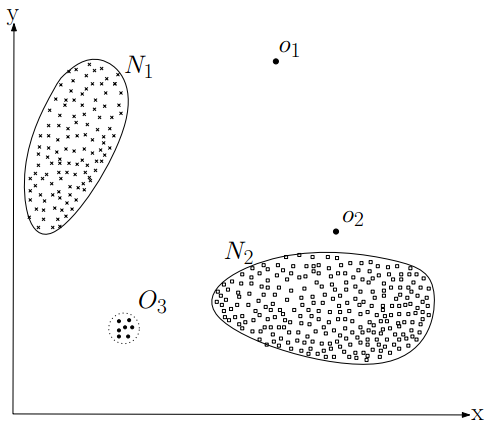
\includegraphics[width=0.5\textwidth]{2d-anomalies}
	\caption[A simple example of anomalies in a 2-dimensional data set.]{A
		simple example of anomalies in a 2-dimensional data set 
		\cite{Chandola:2007}.}
	\label{fig:2d-anomalies}
\end{figure}

% CHALLENGES
\subsection{Challenges}
\label{sec:anomalyDetectionChallenges}
A straightforward anomaly detection approach, is to define a region representing
\singleQuote{normal} behaviour and declare any observation in the data which 
does not belong to this normal region as an anomaly. But several factors make 
this apparently  simple approach very challenging:

\begin{itemize}

\item Defining a normal region which encompasses every possible normal behaviour 
is very difficult. In addition, the boundary between normal and anomalous 
behaviour is often not precise. Thus an anomalous observation which lies close
to the boundary can actually be normal, and vice-versa.

\item When anomalies are the result of malicious actions, the malicious 
adversaries often adapt themselves to make the anomalous observations appear 
like normal, thereby making the task of defining normal behavior more difficult.

\item In many domains normal behavior keeps evolving and a current notion of
normal behavior might not be sufficiently representative in the future.

\item The exact notion of an anomaly is different for different application 
domains. For example, in the medical domain a small deviation from normal (for
example, fluctuations in body temperature) might be an anomaly, while similar 
deviation in the stock market domain (for example, fluctuations in the value of 
a stock) might be considered as normal. Thus applying a technique developed in 
one domain to another is not straightforward.

\item Availability of labeled data for training/validation of models used by 
anomaly detection techniques is usually a major issue.

\item Often the data contains noise which tends to be similar to the actual 
anomalies and hence is difficult to distinguish and remove.

\end{itemize}

Due to the above challenges, the anomaly detection problem, in its most general
form, is not easy to solve. In fact, most of the existing anomaly detection 
techniques solve a specific formulation of the problem. The formulation is 
induced by various factors such as nature of the data, availability of labeled 
data, type of anomalies to be detected, etc. Often, these factors are determined
by the application domain in which the anomalies need to be detected.

Researchers have adopted concepts from diverse disciplines such as statistics, 
data mining, statistics, information theory and spectral theory in order to gain
an increased understanding of anomalies \cite{Chandola:2007}.

% SIMILAR PROBLEMS
\subsection{Similar problems}
\label{sec:similarProblems}
Anomaly detection is an intentionally broad specifier for a class of 
more-specific statisctical challenges. For example, whilst being distinct from, 
anomaly detection is a similar problem (in terms of complexity and approach) to 
that of \emph{noise removal} and \emph{noise accomodation}, both of which are 
aimed at removing the effects of unwanted \emph{noise} in the data. Noise can be
defined as any data which is not of specific interest to the analyst, but in its
presence hinders data analysis techniques \cite{Chandola:2007}. It is often 
critical to data analysis to remove or mitigate the effects that noise has to 
the properties of the host data set.

In contrast, the problem of \emph{novelty detection} can often be impeded by 
techniques that attempt to remove anomalous data from a data set. \emph{Novelty 
detection} is process of discovering emerging patterns in a data set, to provide
an indication of the future state of a system. The distinction between novel
pattern and anomalies is that novel patterns are incorporated into the data 
model after detection \cite{Chandola:2007}.

% CLASSIFICATION
\subsection{Classification}
\label{sec:anomalyClassification}
In general, two different kinds of outliers exist: global outliers and local 
outliers. Global outliers are distinct with respect to the whole data set, while
local outliers are distinct with respect to data points in their local 
neighbourhood \cite{Vries:2011}. The task of global outlier detection has 
undergone much research \citeNeeded{}, but this has not been the case for local 
outlier detection. In the paper \citetitle{Vries:2011}, \citeauthor{Vries:2011} 
optimise the use of local outlier factor (LOF) for large and high-dimensional 
data and propose projection-indexed nearest-neighbours (PINN) --- a novel 
technique that exploits extended nearest-neighbour sets in a reduced-dimensional
space --- to create an accurate approximation for k-nearest-neighbour distances, 
which is used as the core density measurement within LOF \cite{Vries:2011}.

\subsection{Types of anomalies}
\label{sec:typesOfAnomalies}
Anomalies can be classified into three categories \cite{Chandola:2007}:

\begin{description}

\item[Point anomaly] If an individual data instance can be considered as 
anomalous with respect to the rest of data, then the instance is termed as a 
point anomaly. This is the simplest type of anomaly. Referring to 
\autoref{fig:2d-anomalies}, points $o_{1}$ and $o_{2}$, as well as all points in
region $O_{3}$ lie outside the boundary of the normal regions, and are hence 
point anomalies.

\item[Contextual anomalies] If a data instance is anomalous in a certain 
context, but not otherwise, then it is termed a contextual anomaly. The notion 
of a context is induced by the structure in the data set and has to be specified
as part of the problem formulation.

\begin{figure}
	\centering
	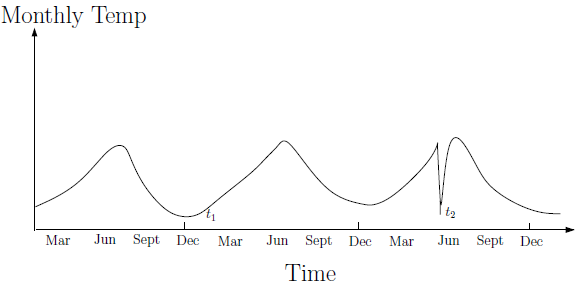
\includegraphics[width=0.5\textwidth]{contextual-anomalies}
	\caption[Contextual anomaly $t_{2}$ in a temperature time series.]{
		Contextual anomaly $t_{2}$ in a temperature time series. Note that the 
		temperature at time $t_{1}$ is same as that at time $t_{2}$ but occurs 
		in a different context and hence is not considered as an anomaly 
		\cite{Chandola:2007}.}
	\label{fig:contextual-anomalies}
\end{figure}

Contextual anomalies have been most commonly explored in time-series data and 
spatial data. \autoref{fig:contextual-anomalies} shows one such example for a 
temperature time series which shows the monthly temperature of an area over last
few years. A temperature of $35\degree F$ might be normal during the winter 
(at time $t_{1}$) at that place, but the same value during summer (at time 
$t_{2}$) would be an anomaly.

\item[Collective anomalies] If a collection of related data instances is 
anomalous with respect to the entire data set, it is termed as a collective 
anomaly. The individual data instances in a collective anomaly may not be 
anomalies by themselves, but their occurrence together as a collection is 
anomalous. \autoref{fig:collective-anomalies} illustrates an example which shows
a human electrocardiogram output. The highlighted region denotes an anomaly 
because the same low value exists for an abnormally long time. Note that that 
low value by itself is not an anomaly.

\begin{figure}
	\centering
	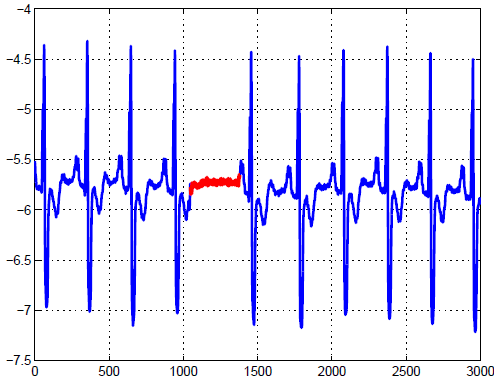
\includegraphics[width=0.5\textwidth]{collective-anomalies}
	\caption[Collective anomaly corresponding to an \emph{Atrial Premature 
		Contraction} in an human electrocardiogram output.]{Collective anomaly 
		corresponding to an \emph{Atrial Premature Contraction} in an human 
		electrocardiogram output \cite{Goldberger:2000}.}
	\label{fig:collective-anomalies}
\end{figure}

\end{description}

% APPROACHES
\subsection{Approaches}

\begin{description}

\item[Classical] A point is declared to be an outlier if its distance from the 
mean is sufficiently large.

\item[Principal Component Analysis] An outlier is usually declared if the point 
is sufficiently far away from the subspace spanned by the eigenvectors 
corresponding to the highest eigenvalues.

\item[Distance based] A point can be declared to be an outlier if its distance 
to its kth nearest-neighbour is sufficiently large.

\item[Statistical based] Statistical methods are often model-based and assume 
that the data should follow some distribution. With knowledge of the 
distribution, data point are evaluated by their fitness to the assumed 
distribution. If the probability of a data instance is less than a certain 
threshold, then that data point is considered an anomaly.

\end{description}

Although distance is an effective non-parametric approach to detecting outliers,
the drawback is the amount of computation time required. Straightforward 
algorithms, such as those based on nested loops, typically require $O(N^{2})$
distance computations. This quadratic scaling means that it will be very 
difficult to mine outliers as we tackle increasingly larger data sets. This is a 
major problem for many real databases where there are often millions of records 
\cite{Bay:2003}.

\subsubsection{Distance based}
In this approach, one looks at the local neighborhood of points for an example 
typically defined by the $k$ nearest examples (also known as neighbours). If the
neighbouring points are relatively close, then the example is considered normal;
if the neighbouring points are far away, then the example is considered unusual.
The advantages of distance-based outliers are that no explicit distribution 
needs to be defined to determine unusualness, and that it can be applied to any 
feature space for which we can define a distance measure \cite{Bay:2003}.

Researchers have tried a variety of approaches to find these outliers 
efficiently. The simplest are those using nested loops \cite{Bay:2003}. In the 
basic version one compares each example with every other example to determine 
its $k$ nearest neighbors. Given the neighbors for each example in the data set,
simply select the top $n$ candidates according to the outlier definition. This 
approach has quadratic complexity as we must make all pairwise distance 
computations between examples.

Another method for finding outliers is to use a spatial indexing structure such 
as a KD-tree, R-tree, or X-tree to find the nearest neighbors of each candidate 
point. One queries the index structure for the closest $k$ points to each 
example, and as before one simply selects the top candidates according to the 
outlier definition. For low-dimensional data sets this approach can work 
extremely well and potentially scales as $O(N \log N)$ if the index tree can
find an example's nearest neighbors in $\log N$ time. However, index structures 
break down as the dimensionality increases \cite{Bay:2003}.

\subsubsection{Statistical based}
A common distribution considered when modelling data is the \singleQuote{Normal}
distribution. Using this model, the probability that a data instance lies within
$k$ standard deviations $\sigma$ from the mean $\mu$ is the area between 
$\mu - k\sigma$ and $\mu + k\sigma$.

% LOCAL OUTLIER FACTOR
\subsection{Local Outlier Factor}
\label{sec:localOutlierFactor}
\singleQuote{Local Outlier Factor} is a formula that captures the degree to 
which a data point is an outlier with respect to its local neighbourhood. In 
this context, \singleQuote{local} means that the determination of the data 
points does not depend on knowledge of the global distribution of the data set.


%%%%%%%%%%%%%%%%%%%%%%%%%%%%%%%%%%%%%%%%%%%%%%%%%
% Distance Metrics
%%%%%%%%%%%%%%%%%%%%%%%%%%%%%%%%%%%%%%%%%%%%%%%%%
\section{Distance Metrics}
\label{distanceMetrics}
Distance is a quantitative description of how far apart two objects are.
Mathematically, a distance or metric is a function describing how close or far
away data points in some space are from each other \cite{Khoa:2012}.

%%%%%%%%%%%%%%%%%%%%%%%%%%%%%%%%%%%%%%%%%%%%%%%%%%%%%%%%%%%%%%%%%%%%%%%%%%%%%%%%
% Euclidean Distance
%%%%%%%%%%%%%%%%%%%%%%%%%%%%%%%%%%%%%%%%%%%%%%%%%%%%%%%%%%%%%%%%%%%%%%%%%%%%%%%%
\subsection{Euclidean Distance}
\label{euclidianDistance}
An Euclidean distance between two data points in a space is the norm of the
difference between two vectors corresponding to these data points
\cite{Khoa:2012}. Euclidean distance is extremely sensitive to the scale of the
features involved. When dealing with features of vastly different scales, the
effects of the larger feature dominant over the smaller feature in terms of the
Euclidean distance. This problem is usually solved by normalizing the data
values. Another issue, however, with Euclidean distance is that it is unable to
take into account any correlation between data features.

%%%%%%%%%%%%%%%%%%%%%%%%%%%%%%%%%%%%%%%%%%%%%%%%%%%%%%%%%%%%%%%%%%%%%%%%%%%%%%%%
% Mahalanobis Distance
%%%%%%%%%%%%%%%%%%%%%%%%%%%%%%%%%%%%%%%%%%%%%%%%%%%%%%%%%%%%%%%%%%%%%%%%%%%%%%%%
\subsection{Mahalanobis Distance}
\label{mahalanobisDistance}
Mahalanobis distance is a distance measure that considers the covariance between
data features. Mahalanobis distance, however, is extremely sensitive to
anomalies as anomalies affect both the mean and the covariance of the data.

%%%%%%%%%%%%%%%%%%%%%%%%%%%%%%%%%%%%%%%%%%%%%%%%%%%%%%%%%%%%%%%%%%%%%%%%%%%%%%%%
% Graph Geodesic Distance
%%%%%%%%%%%%%%%%%%%%%%%%%%%%%%%%%%%%%%%%%%%%%%%%%%%%%%%%%%%%%%%%%%%%%%%%%%%%%%%%
\subsection{Graph Geodesic Distance}
\label{graphGeodesicDistance}
% TODO

%%%%%%%%%%%%%%%%%%%%%%%%%%%%%%%%%%%%%%%%%%%%%%%%%
% Vectors and Matrices
%%%%%%%%%%%%%%%%%%%%%%%%%%%%%%%%%%%%%%%%%%%%%%%%%
\section{Vectors and Matrices}
\label{vectorsAndMatrices}
%%%%%%%%%%%%%%%%%%%%%%%%%%%%%%%%%%%%%%%%%%%%%%%%%
% Eigenvectors and Eigenvalues
%%%%%%%%%%%%%%%%%%%%%%%%%%%%%%%%%%%%%%%%%%%%%%%%%
\subsection{Eigenvectors and Eigenvalues}
\label{eigenvectors}
\label{eigenvalues}
This section will briefly recall some basic definitions of eigenvectors and
eigenvalues, as well as some of their basic properties.

A vector $\mathbf{v}$ is an eigenvector of a matrix $M$ of eigenvalue $\lambda$
if:
\begin{equation}
M\mathbf{v} = \lambda\textbf{v}
\end{equation}

If $\mathbf{v_1}$ is an eigenvector of $M$ of eigenvalue $\lambda_1$,
$\mathbf{v_2}$ is an eigenvector of $M$ of eigenvalue $\lambda_2\neq\lambda_1$,
and $M$ is symmetric, then $\mathbf{v_1}$ is orthogonal to $\mathbf{v_2}$.

For a symmetric matrix $M$, the multiplicity of an eigenvalue $\lambda$ is the
dimension of the space of eigenvectors of eigenvalue $\lambda$. Also recall that
every $n\times n$ symmetric matrix has $n$ eigenvalues, counted with
multiplicity. Thus, it has an orthonormal basis of eigenvectors,
$\begin{Bmatrix} \mathbf{v_1} & \ldots & \mathbf{v_n} \end{Bmatrix}$ with
eigenvalues $\lambda_1\leq\lambda_2\leq\ldots\leq\lambda_3$ so that:
\begin{equation}
M\mathbf{v_i} = \lambda_i \mathbf{v_i} \quad \forall i
\end{equation}

If we let $V$ be the matrix whose $i$th column is $v_i$ and $\Lambda$ be the
diagonal matrix whose $i$th diagonal is $\lambda_i$, we can write this more
compactly as:
\begin{equation}
MV = V\Lambda
\end{equation}

Multiplying by $V^T$ on the right, we obtain the eigen-decomposition of $M$:
\begin{equation}
M = MVV^T = V{\Lambda}V^T = \sum_i \lambda_i\mathbf{v_i}\mathbf{v_i^T}
\end{equation}

%%%%%%%%%%%%%%%%%%%%%%%%%%%%%%%%%%%%%%%%%%%%%%%%%
% Eigen Decomposition
%%%%%%%%%%%%%%%%%%%%%%%%%%%%%%%%%%%%%%%%%%%%%%%%%
\subsection{Eigen Decomposition}
\label{eigenDecomposition}
% TODO

%%%%%%%%%%%%%%%%%%%%%%%%%%%%%%%%%%%%%%%%%%%%%%%%%
% Laplacian Matrices
%%%%%%%%%%%%%%%%%%%%%%%%%%%%%%%%%%%%%%%%%%%%%%%%%
\subsection{Laplacian Matrices}
\label{laplacianMatrices}
\nocite{Berkeley:1999,Pati:2011,Spielman:2006}
Recall that a weighted, undirected graph $G = (V,E,w)$ is essentially an
undirected graph $G = (V,E)$ along with a function $w : E \rightarrow \Re^+$,
where $\Re^+$ denotes the set of positive real numbers.

The adjacency matrix of a weighted graph $G$ is be denoted $A_G$, and is given
by:
\begin{equation}
A_{G}(i,j) :=
    \left\{
        \begin{array}{ll}
            \mathit{w}(i,j) &   \quad \text{if $(i,j) \in E$}\\
            0 &                 \quad \text{otherwise}
        \end{array}
    \right.
\end{equation}

The degree matrix of a weighted graph $G$, denoted $D_G$, is the diagonal matrix
such that:
\begin{equation}
D_G(i,i) = \sum_j A_G(i,j)
\end{equation}

A Laplacian Matrix is a matrix representation of a graph, defined by the
equation:
\begin{equation}
L_G = D_G - A_G
\end{equation}

For a vector $\textbf{x} \in \Re^V$, the Laplacian quadratic form of $G$ is:
\begin{equation}
\label{laplacianQuadraticForm}
\textbf{x}^T L \textbf{x} = \sum_{(u,v) \in E} w_{u,v}(\textbf{x}(u) - \textbf{x}(v))^2
\end{equation}

From \autoref{laplacianQuadraticForm}, it can be seen that $L$ provides a
measure of the smoothness of $\textbf{x}$ over the edges in $G$. The more
$\textbf{x}$ jumps over an edge, the larger the quadratic form becomes.

It is often more convenient to consider the normalized Laplacian of a graph
instead of the Laplacian \cite{Spielman:2010}. The normalized Laplacian is given
by $D^{-1/2}LD^{-1/2}$ and is more closely related to the behaviour of random
walks.

Now, let $G_{1,2}$ be a graph on two vertices with a single edge of weight $1$.
\begin{equation}
L_{G_{1,2}} :=
    \begin{bmatrix}
        1 & -1\\
        -1 & 1
    \end{bmatrix}
\end{equation}

For the graph with $n$ vertices and just one edge between vertices $u$ and $v$,
we can define the Laplacian Matrix similarly. For concreteness, I'll call this
graph $G_{u,v}$. It's Laplacian Matrix is the $n \times n$ matrix whose only
non-zero entries are in the intersections of rows and columns $u$ and $v$. The
$2 \times 2$ matrix at the intersections of these rows and columns is, of
course:
\begin{equation}
    \begin{bmatrix}
        1 & -1\\
        -1 & 1
    \end{bmatrix}
\end{equation}

For a weighted graph $G = (V,E,w)$, we define:
\begin{equation}
L_G := \sum_{(u,v) \in E} w(u,v)L_{G_{u,v}}
\end{equation}

% Properties
\subsubsection{Properties}
\label{laplacianMatrices:properties}
Laplacian matrices of graphs are symmetric, have zero row-sums, and have
nonpositive off-diagonal entries. We call any matrix that satisfies these
properties a Laplacian matrix, as there always exists some graph for which it is
the Laplacian \cite{Spielman:2010}.

For a graph $G$ and its Laplacian Matrix $L$ with eigenvalues $\lambda_0<
\lambda_1<\ldots<\lambda_{n-1}$:

\begin{itemize}
\item $L$ is a symmetric matrix. This means the eigenvalues of $L$ are real, and
its eigenvectors are real and orthogonal.
\item $L$ is always positive-semidefinite ($\forall i,\lambda_i\geq 0;
\lambda_0=0$).
\item Let $G=(V,E)$ be a graph, and let $0=\lambda_1\leq\lambda_2\leq\ldots\leq
\lambda_n$ be the eigenvalues of its Laplacian Matrix. Then, $\lambda_2>0$ if
and only if $G$ is connected.
\item The number of times $0$ appears as an eigenvalue in the Laplacian Matrix
is the number of connected components in the graph.
\item $\lambda_0$ is always $0$ because every Laplacian Matrix has an
eigenvector of $\begin{bmatrix} 1 & 1 & \ldots & 1 \end{bmatrix}$ that, for each
row, adds the corresponding node's degree to a ``-1'' for each neighbour,
thereby producing zero by definition.
\item The smallest non-zero eigenvalue of $L$ is called the spectral gap.
\item If we arbitrarily assign an orientation to the edges in $G$ and label each
edge, then we can define the vertex edge incidence matrix $Q$ by:
\begin{equation}
Q_{ij} := 
    \left\{
        \begin{array}{ll}
            1 &     \quad \text{if $e_j$ starts from $i$}\\
            -1 &    \quad \text{if $e_j$ ends at $i$}\\
            0 &     \quad \text{otherwise}
        \end{array}
    \right.
\end{equation}
Then the Laplacian Matrix $L$ satisfies $L = Q^TQ$, regardless of the
orientation of the edges.
\item The second smallest eigenvalue of $L$ ($\lambda_2$) is the algebraic
connectivity of $G$. $\lambda_2>0$ if and only if $G$ is connected.
\end{itemize}

% Applications
\subsubsection{Applications}
\label{laplacianMatrices:applications}
An interesting application of Laplacian matrices is that of modelling electrical
flow in a network resistors. In this model, the vertices of the graph correspond
to points at which current can be added to or removed from the circuit. Edges in
the graph correspond to resistors, with the edge weight equal to the conductance
of the electrical resistor.

If $\textbf{p} \in \Re^V$ denotes the vector of potentials and $\textbf{i}_{ext}
\in \Re^V$ the vectors of currents entering and leaving vertices, then these
satisfy the relation:
\begin{equation}
L\textbf{p} = \textbf{i}_{ext}
\end{equation}

This equation can be exploited to compute the effective resistance between
pairs of vertices \cite{Spielman:2010}. The effective resistance between
vertices $u$ and $v$ is the difference in potential one must impose between $u$
and $v$ to flow one unit of current from $u$ to $v$. To measure this, we compute
the vector $\textbf{p}$ for which $L\textbf{p} = \textbf{i}_{ext}$, where:
\begin{equation}
\textbf{i}_{ext}(x) =
    \left\{
        \begin{array}{ll}
            1 &     \quad \text{for $x=u$}\\
            -1 &    \quad \text{for $x=v$}\\
            0 &     \quad \text{otherwise}
        \end{array}
    \right.
\end{equation}

We then measure the difference between $\textbf{p}(u)$ and $\textbf{p}$(v).


%%%%%%%%%%%%%%%%%%%%%%%%%%%%%%%%%%%%%%%%%%%%%%%%%
% Markov Chains
%%%%%%%%%%%%%%%%%%%%%%%%%%%%%%%%%%%%%%%%%%%%%%%%%
\section{Markov Chains}
\label{markovChains}
A \singleQuote{Markov chain} is a chance process in which the outcome of a given
experiment can affect the outcome of the next experiment \cite{Grinstead:1997}. 
For a Markov chain, we have a set of states $S = \left\{ s_{1}, s_{2}, \ldots, 
s_{r} \right\}$ with a process starting in one of the states and moving from 
state $s_{i}$ to $s_{j}$ with a probability $p_{ij}$ not dependent upon which 
states the chain was in before the current state. The probabilities $p_{ij}$ are
called \emph{transition probabilities}, and the complete matrix $\mathbf{P}$ of 
probabilities is known as the \emph{transition matrix}.

The probability that, given the chain is in state $i$ now, it will be in state 
$j$ in two steps is denoted by $p_{ij}^{(2)}$. In general, if a Markov chain has 
$r$ states, then:

\begin{equation}
p_{ij}^{(2)} = \sum_{k=1}^{r} p_{ik}p{kj}
\end{equation}


%%%%%%%%%%%%%%%%%%%%%%%%%%%%%%%%%%%%%%%%%%%%%%%%%
% Random Projections
%%%%%%%%%%%%%%%%%%%%%%%%%%%%%%%%%%%%%%%%%%%%%%%%%
\section{Random Projections}
\label{randomProjections}
% TODO

%%%%%%%%%%%%%%%%%%%%%%%%%%%%%%%%%%%%%%%%%%%%%%%%%
% Random Walks and Commute Time
%%%%%%%%%%%%%%%%%%%%%%%%%%%%%%%%%%%%%%%%%%%%%%%%%
\section{Random Walks and Commute Time}
\label{randomWalks}
\label{commuteTime}
Assume we are given a connected undirected and weighted graph $G=(V,E,W)$ with
edge weights $(w_{ij})_{i,j \in V}>=0$ be the graph adjacency matrix. A degree
of a node $i$ is $d_i=\sum_{j\in N(i)}w_{ij}$ where $N(i)$ is a set of
neighbours of node $i$. All nodes nonadjacent to $i$ are assumed to have a
weight of $w_{ij}=0$.

A random walk is a sequence of nodes on a graph visited by a random walker:
starting from a node, the random walker moves to one of its neighbours with some
probability. Then from that node, it proceeds to one of its own neighbours with
some probability, and so on \cite{Khoa:2012}. The random walk is a finite Markov
chain that is time-reversible, which means the reverse Markov chain has the same
transition probability matrix as the original Markov chain \cite{Lovasz:1996}.

The probability that a random walker selects a particular node from is
neighbours is determined by the edge weights of the graph. The larger the weight
$w_{ij}$ of the edge connecting nodes $i$ and $j$, the more often the random
walker travels through that edge.

%%%%%%%%%%%%%%%%%%%%%%%%%%%%%%%%%%%%%%%%%%%%%%%%%
% Similarity Graphs
%%%%%%%%%%%%%%%%%%%%%%%%%%%%%%%%%%%%%%%%%%%%%%%%%
\subsection{Similarity Graphs}
\label{similarityGraphs}
% TODO

%%%%%%%%%%%%%%%%%%%%%%%%%%%%%%%%%%%%%%%%%%%%%%%%%
% Hitting Time
%%%%%%%%%%%%%%%%%%%%%%%%%%%%%%%%%%%%%%%%%%%%%%%%%
\subsection{Hitting Time}
\label{hittingTime}
% TODO

%%%%%%%%%%%%%%%%%%%%%%%%%%%%%%%%%%%%%%%%%%%%%%%%%
% Commute Time
%%%%%%%%%%%%%%%%%%%%%%%%%%%%%%%%%%%%%%%%%%%%%%%%%
\subsection{Commute Time}
\label{commuteTime}

% Introduction
\subsubsection{Introduction}
\label{commuteTime:introduction}
Commute time is a robust distance metric derived from a random walk on graphs
\cite{Khoa:2012}. In \citetitle{Khoa:2012}, \citeauthor{Khoa:2012} demonstrated
how commute time can be used as a distance measure for data mining tasks such as
anomaly detection and clustering. A prohibitive limitation of this technique is
that the calculation of commute time involves the eigen decomposition of the
graph Laplacian, making it impractical for large graphs.

A major advantage of using commute time as a distance metric for outlier
detection is that it effectively captures not only the distances between data
points but also the density of the data \citeNeeded{}. This property results in
a distance metric that can be effectively used to capture global, local and
group anomalies.

The commute time between two nodes $i$ and $j$ in a graph is the number of steps
that a random walk, starting from $i$ will take to visit $j$ and then come back
to $i$ for the first time. The fact that the commute time is averaged over all
paths (and not just the shortest path) makes it more robust to data
perturbations and it can also capture graph density \cite{Khoa:2012}. Since it
is a measure which can capture the geometrical structure of the data and is
robust to noise, commute time can be applied in methods where Euclidean or other
distances are used and thus the limitations of these metrics can be avoided.

% Limitations
\subsubsection{Limitations}
\label{commuteTime:limitations}
The computation of commute time requires the eigen decomposition (see
\autoref{eigenDecomposition}) of the graph Laplacian matrix (see
\autoref{laplacianMatrices}), a computation which takes $O(n^3)$ time and thus
is not practical for large graphs \citeNeeded{}. Methods to approximate the
commute time to reduce the computational time are required in order to
efficiently use commute time in large datasets.


%%%%%%%%%%%%%%%%%%%%%%%%%%%%%%%%%%%%%%%%%%%%%%%%%
% Nearest Neighbour Algorithms
%%%%%%%%%%%%%%%%%%%%%%%%%%%%%%%%%%%%%%%%%%%%%%%%%
\section{Nearest Neighbour Algorithms}
\label{nearestNeighbourAlgorithms}
% TODO

%%%%%%%%%%%%%%%%%%%%%%%%%%%%%%%%%%%%%%%%%%%%%%%%%
% Solvers
%%%%%%%%%%%%%%%%%%%%%%%%%%%%%%%%%%%%%%%%%%%%%%%%%
\section{Solvers}
\label{solvers}
% SPIELMAN-TENG SOLVER
\subsection{Spielman-Teng Solver}
\label{sec:spielmanTengSolver}
\nocite{Spielman:2006}
Spielman and Teng presented a randomised algorithm that, on input a symmetric,
weakly diagonally dominant $n{\times}x$ matrix $A$ with $m$ non-zero entries and
an $n$-vector $\mathbf{b}$, produces an $\tilde{\mathbf{x}}$ such that
$\begin{Vmatrix} \tilde{\textbf{x}} - A^{\dagger}\textbf{b} \end{Vmatrix}_{A}
\leq \epsilon \begin{Vmatrix} A^{\dagger}\mathbf{b} \end{Vmatrix}_{A}$ in
expected time:
\begin{equation}
m \log^{O(1)} n \log (1/\epsilon)
\end{equation}


%%%%%%%%%%%%%%%%%%%%%%%%%%%%%%%%%%%%%%%%%%%%%%%%%
% Anomaly Detection Using Commute Time
%%%%%%%%%%%%%%%%%%%%%%%%%%%%%%%%%%%%%%%%%%%%%%%%%
\section{Anomaly Detection Using Commute Time}
\label{anomalyDetection:commuteTime}
% INTRODUCTION
\subsection{Introduction}
\label{commuteTime:introduction}
Commute time is a robust distance metric derived from a random walk on graphs
\cite{Khoa:2012}. In \citetitle{Khoa:2012}, \citeauthor{Khoa:2012} demonstrated
how commute time can be used as a distance measure for data mining tasks such as
anomaly detection and clustering. A prohibitive limitation of this technique is
that the calculation of commute time involves the eigen decomposition of the
graph Laplacian, making it impractical for large graphs.

A major advantage of using commute time as a distance metric for outlier
detection is that it effectively captures not only the distances between data
points but also the density of the data \citeNeeded. This property results in a
distance metric that can be effectively used to capture global, local and group
anomalies.

The commute time between two nodes $i$ and $j$ in a graph is the number of steps
that a random walk, starting from $i$ will take to visit $j$ and then come back
to $i$ for the first time. The fact that the commute time is averaged over all
paths (and not just the shortest path) makes it more robust to data
perturbations and it can also capture graph density \cite{Khoa:2012}. Since it
is a measure which can capture the geometrical structure of the data and is
robust to noise, commute time can be applied in methods where Euclidean or other
distances are used and thus the limitations of these metrics can be avoided.

% LIMITATIONS
\subsection{Limitations}
\label{commuteTime:limitations}
The computation of commute time requires the eigen decomposition (see
\autoref{sec:eigenDecomposition}) of the graph Laplacian matrix (see
\autoref{sec:laplacianMatrices}), a computation which takes $O(n^{3})$ time and
thus is not practical for large graphs \citeNeeded. Methods to approximate the
commute time to reduce the computational time are required in order to
efficiently use commute time in large datasets.

% ANOMALY DETECTION USING COMMUTE TIME
\subsection{Anomaly Detection Using Commute Time}
\label{commuteTime:anomalyDetection}
% TODO



\end{document}
